\section{Carbon Footprint and Federal Leadership}
\textit{Deborah Weighill}

\subsection{Introduction}
This section will discuss Greenhouse Gas (GHG) and carbon emissions of the Federal government, how our policy fits in with existing Federal initiatives to lower carbon emissions, as well as analyze the potential affect our policy could have in reducing Federal building carbon emissions.

\subsection{Greenhouse Gas Emissions of the USA and the Federal Government}
Greenhouse gases (GHGs) are gases that contribute to climate change. Since there are a variety of such gases (not only CO$_{2}$) GHG emissions are measured in terms of equivalent Global Warming Potential (GWP), with CO$_{2}$ as the reference gas. For a given weight of a particular greenhouse gas, the equivalent weight of CO$_{2}$ is the weight of CO$_{2}$ which has the same GWP as the weight of the original gas. Thus, the total GHG emissions are measured as the sum of the weights of the gases measured in the equivalent weight of CO$_{2}$ \cite{debbie}{1}.
\\\\
\noindent Under Executive Order 13514 \cite{debbie}{2}, government agencies were required to report GHG emissions. These reports were released for the first time in 2011. The Federal Government's total GHG emissions were 123.2 Million Metric Tonnes of CO$_{2}$ Equivalent (MMTCO2 Equiv) in 2011 \cite{debbie}{3}. However, only half of these which are subject to reduction targets are adequately reported on \cite{debbie}{4, 5}. To put this figure in context, the total GHG emissions of the whole of the United States was 6843 MMTCO2 Equiv in 2011 \cite{debbie}{1}. The GHG emissions for the US up until the year 2013 are visualized in Figures \ref{d1} \cite{debbie}{1} and \ref{d2} \cite{debbie}{6}. Figure \ref{d1} clearly shows that the GHG emissions are dominated by CO$_{2}$, with the other GHGs contributing a minorly. Approximately one third of the carbon emissions of the US is due to electricity generation \cite{newfigsepa2}.

\begin{figure}
\begin{center}
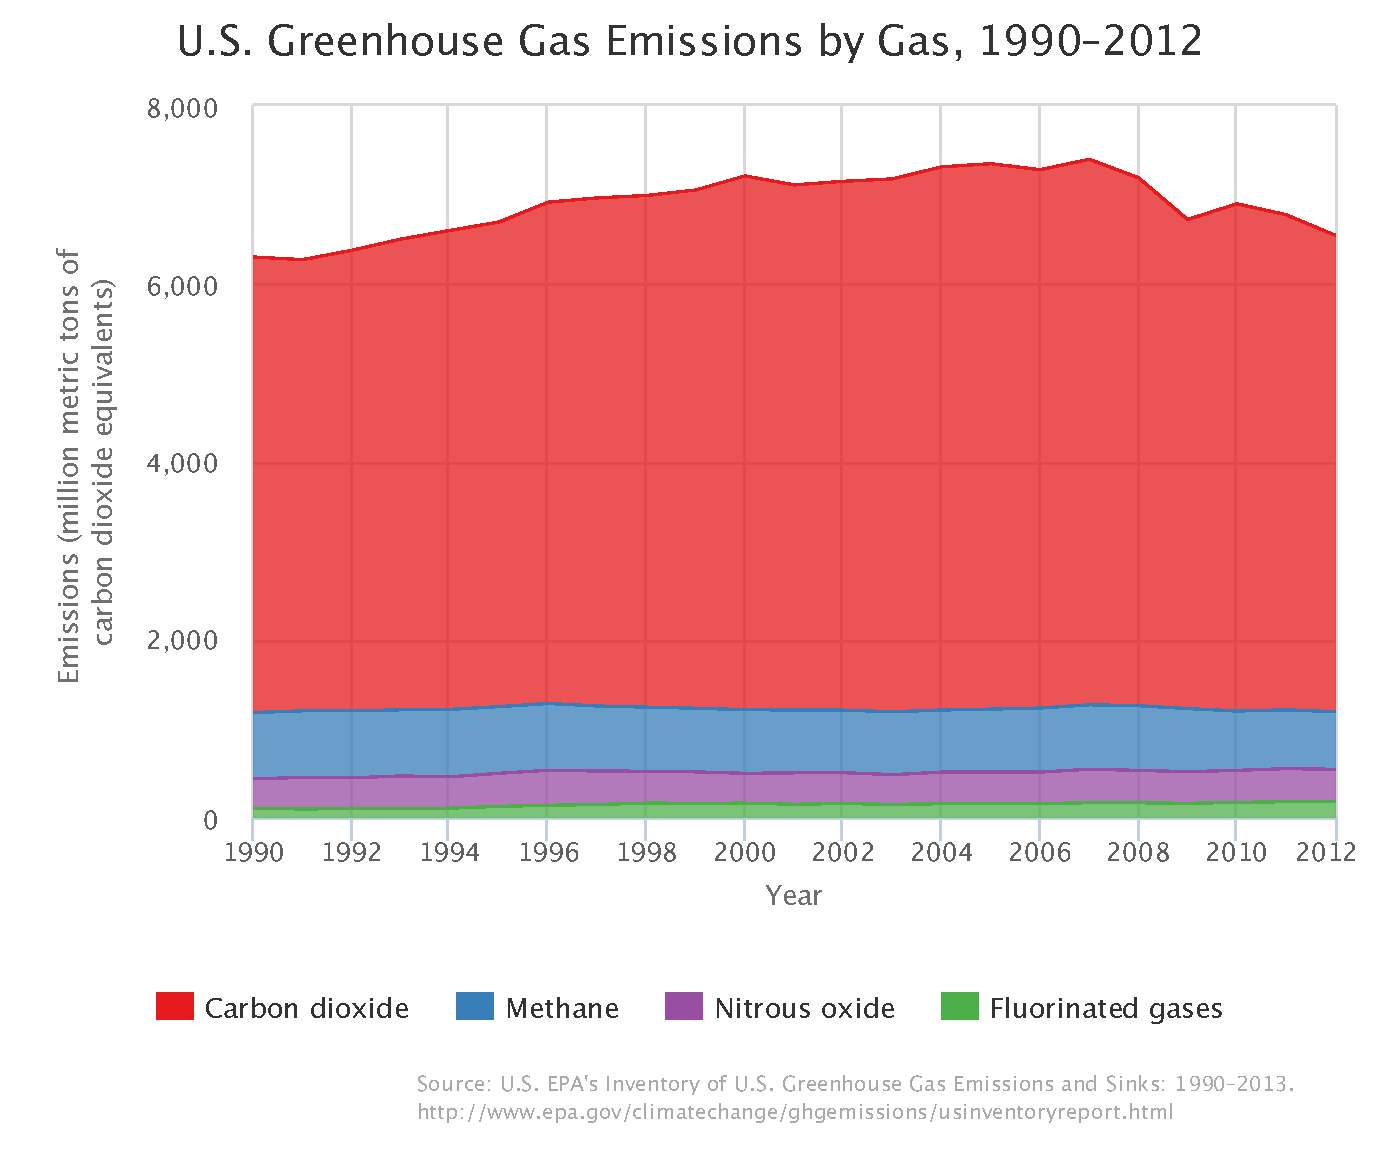
\includegraphics[scale=0.6]{pics/new_d1.pdf}
\caption{GHG Emissions of the USA. (Figure from \cite{debbie}{newfigsepa})}
\label{d1}
\end{center}
\end{figure}

\begin{figure}
\begin{center}
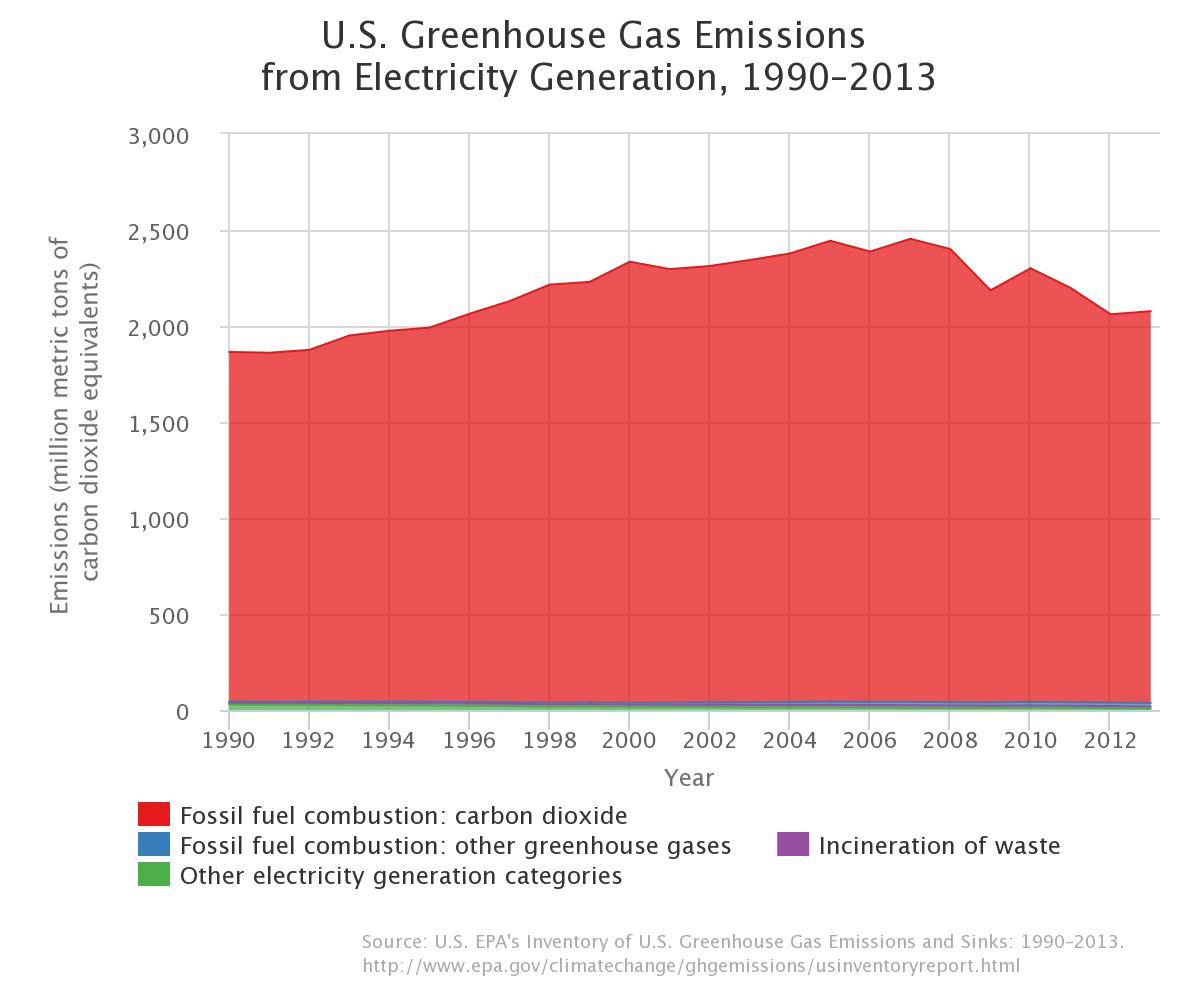
\includegraphics[scale=0.35]{pics/chart.png}
\caption{GHG Emissions due to Electricity of the USA. (Figure from \cite{debbie}{newfigsepa2})}
\label{d1}
\end{center}
\end{figure}

\begin{figure}
\begin{center}
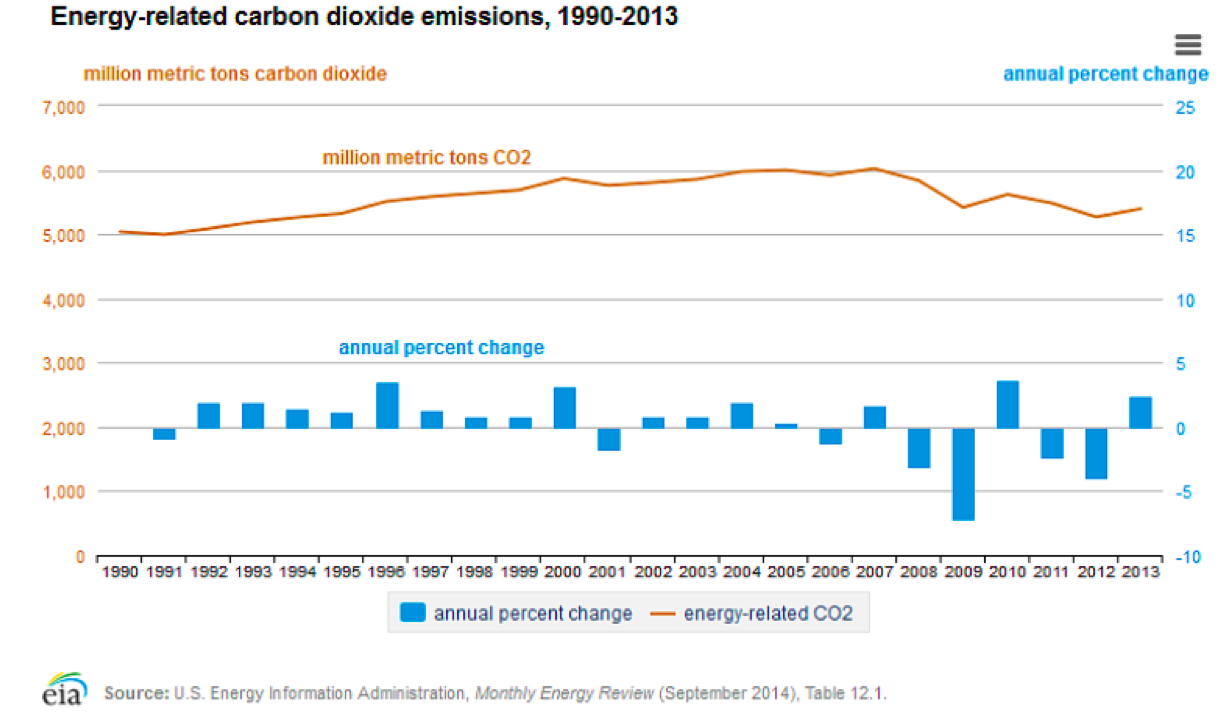
\includegraphics[scale=0.3]{pics/d2.png}
\caption{CO$_{2}$ emissions and annual percent change of CO$_{2}$ emissions of the USA. (Figure from \cite{debbie}{2})}
\label{d2}
\end{center}
\end{figure}

\subsection{Addressing Existing Government Initiatives}
In this section, we highlight how our policy addresses goals within existing government policies.

\paragraph{Executive Order 13514 - Federal Leadership in Environmental, Energy, and Economic Performance} 
\mbox{  }\\
On 5 October 2009, President Obama released Executive Order 13514: Federal Leadership in Environmental, Energy and Economic Performance \cite{debbie}{2}. The purpose of this order was to promote clean and sustainable energy, and that the Federal government should lead by example through improving their energy efficiency, lowering their GHG emissions and measuring and openly reporting their progress towards these goals.
\\\\
\noindent Implementation of our policy would address several of the specific instructions given in this executive order. Section 2(b)(i) of this order directs Federal agencies to consider achieving GHG reductions by \textit{``pursuing opportunities with vendors and contractors to address and incorporate incentives to reduce greenhouse gas emissions...''} \cite{debbie}{2}. Our policy recommendation provides a means to address this by choosing vendors producing the most energy efficient and carbon efficient solar panels to install their panels on the roofs of Federal buildings.
\\\\
\noindent Our policy also addresses Section 2(g)(i) of the Executive Order, which stipulates that \textit{``beginning in 2020 and thereafter, ensuring that all new Federal buildings that enter the planning process are designed to achieve zero net-energy by 2030''}. Installing efficient solar panel on the roofs of Federal buildings will contribute to them being energy neutral. Similarly, our policy addresses Section 2(a)(ii), which involves \textit{``increasing agency use of renewable energy and implementing renewable energy generation projects on agency property ''} \cite{debbie}{2}.
\\\\
\noindent In response to Executive Order 13514, the GreenGov Initiative was launched \cite{debbie}{7}. This initiative called upon all government employees to share ideas about how the goals set out in the Executive Order could be achieved. The top voted ideas were summarized in a report which was released in February 2010 \cite{debbie}{8}. In this report, one of the top-voted ideas by government employees was the installation of solar panels on government buildings.

\paragraph{President Obama's Climate Action Plan} \mbox{ }\\
In June 2013, President Obama’s Climate Action Plan was released. The three main ``pillars'' of this plan were: 1) cutting carbon emissions, 2) preparing for the impacts of climate change, and 3) leading international efforts to against climate change \cite{debbie}{9, 10, 11}. Our policy directly addresses two of the goals in this Climate Action Plan, namely the goal aiming to double the amount of wind and solar energy produced in the USA by the year 2020, and the second aiming to have 20\% of the Federal Government’s energy demands coming from renewable sources \cite{debbie}{11}.

\paragraph{Executive Order 13693 - Planning for Federal Sustainability in the Next Decade} \mbox{ }\\
Very recently, on 19 March 2015, Executive Order 13693 was issued
\cite{debbie}{12}. This Executive Order included very specific goals for GHG emission reduction. Section 3(c) stipulated that 10\% of electricity usage by Federal Agencies had to be generated from renewable sources by 2016, 15\% by 2018, 20\% by 2020, 25\% by 2022 and 30\% by 2025 \cite{debbie}{12}. Section 3(d)(i) stated that Government Agencies should attempt to reach these goals by installing renewable energy sources on site at the Federal facilities \cite{debbie}{12}. These orders would be directly addressed through the implementation of our policy.

\subsection{GHG Emissions from PV Cells}
PV cells do not, that we know of, produce any GHGs specifically by making electricity, however, GHG’s are produced during activities at all stages of the PV cell’s lifetime \cite{debbie}{13}. The analysis of the GHG’s produced throughout the whole lifetime of the PVC, from resource acquisition and manufacture to decommissioning and disposal, is known as Life Cycle Analysis (LCA). The main steps in the lifecycle of a PVC, as well as the approximate percentage of GHG emission at each stage are shown in Figure \ref{d3} \cite{debbie}{14}.
\\\\
\noindent A literature study was performed, aggregating the results of many LCA analyses of PVCs. The resulting lifecycle carbon intensities of the PVCs (measured in grams CO$_{2}$equiv/kWh) had a very broad range, as seen in Figure \ref{d4} \cite{debbie}{13}. However, even with this large range, the GHG emissions from PVCs are still significantly lower than that of coal (Figure \ref{d5} \cite{debbie}{15}).

\begin{figure}
\begin{center}
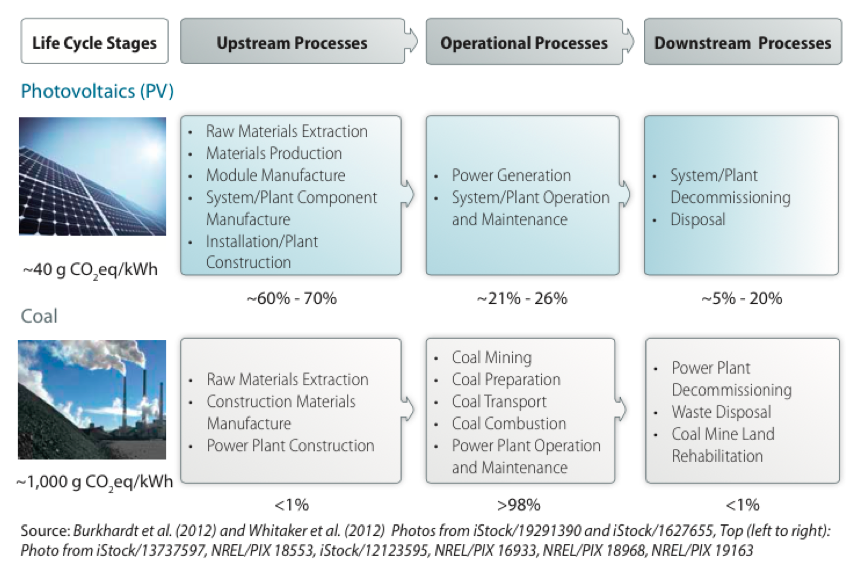
\includegraphics[scale=0.4]{pics/d3.png}
\caption{Stages in LCA of PVCs, and the relative contribution of each stage to the total GHG emissions of PVCs. (Figure from \cite{debbie}{14})}
\label{d3}
\end{center}
\end{figure}

\begin{figure}
\begin{center}
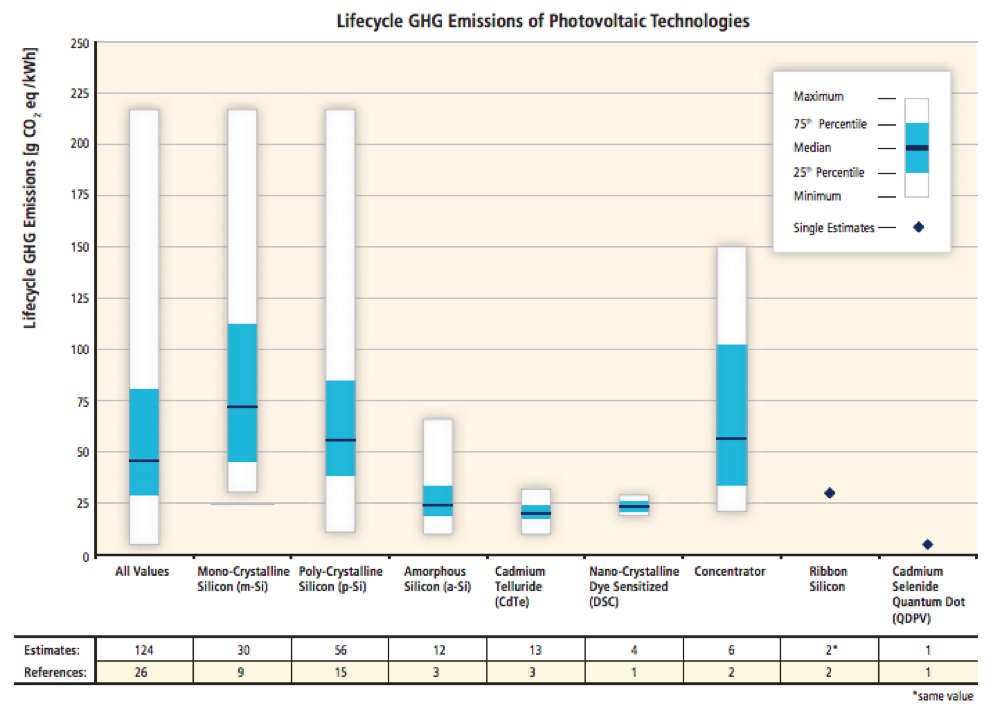
\includegraphics[scale=0.35]{pics/d4.png}
\caption{LCA GHG emissions from different PV technologies. (Figure from \cite{debbie}{13})}
\label{d4}
\end{center}
\end{figure}

\begin{figure}
\begin{center}
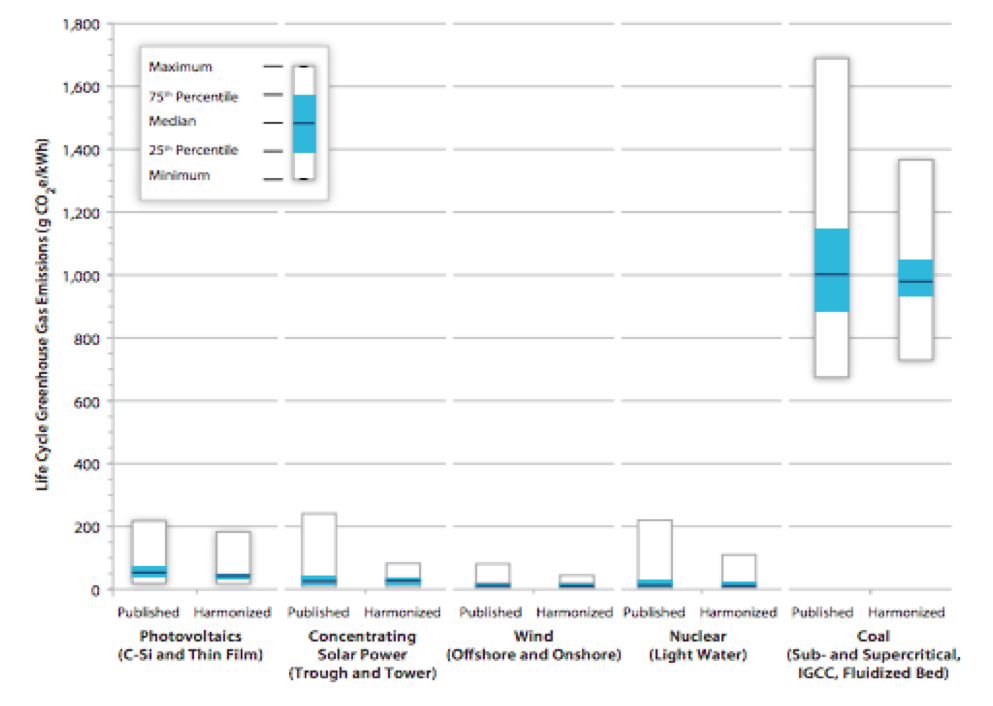
\includegraphics[scale=0.35]{pics/d5.png}
\caption{LCA GHG emissions from different energy sources. (Figure from \cite{debbie}{15})}
\label{d5}
\end{center}
\end{figure}

\subsection{Carbon Emission Analysis}
We performed a Carbon Emissions analysis to attempt to estimate the effect this policy could potentially have on Federal carbon emissions. The Federal Government consists of more than 360,000 buildings \cite{debbie}{7}. As a sample for this analysis, all documented U.S. General Services Administration (GSA) buildings were used.

\begin{table}
\begin{center}
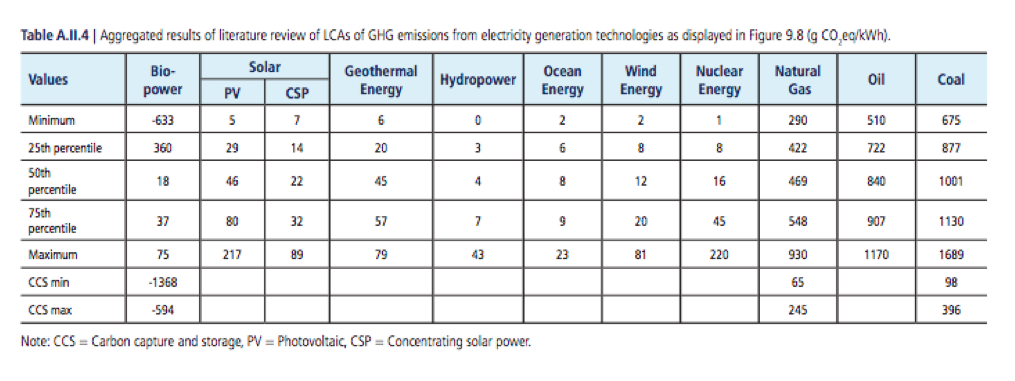
\includegraphics[scale=0.43]{pics/t1.png}
\caption{Solar LCA GHG Emissions. (Table from \cite{debbie}{13})}
\label{t1}
\end{center}
\end{table}

\paragraph{Resources for Carbon Analysis} \mbox{ }\\
A database of all GSA Federal buildings was compiled which also included an estimate of solar insolence at each building, electricity demand of each building, rooftop area and solar energy potential (Compiled by Roison Langan using \cite{debbie}{roisin}). The carbon intensity (mass of carbon dioxide produced per unit energy) for each state was obtained from an energy report published by the U.S. Energy Information Administration (EIA) in August 2014 \cite{debbie}{16}. There was no data available on GHG intensity (mass of all greenhouse gases produced per kWh) at a state-level resolution. A report by the Intergovernmental Panel on Climate Change reported agglomerated GHG emission from various LCA studies of PV panels \cite{debbie}{13}. The values given by this study are in grams CO$_{2}$ equivalents, and thus theoretically contain gases other than CO$_{2}$, however, it has been noted in various sources \cite{debbie}{17, 18} that in LCA studies of PV cells, the major component of GHG emissions is CO$_{2}$. We thus justify using these GHG intensity figures (grams CO$_{2}$ equiv/kWh) as an approximation of the carbon intensity (grams CO2/kWh).

\paragraph{Carbon Analysis Methods} \mbox{ }\\
For each Federal building $B$, the solar potential $P_{{\mbox{solar}}_{B}}$ (kWh/day) was defined as the maximum amount of solar energy which could be produced by the building through rooftop solar panels. This was calculated as:

\begin{equation}
P_{{\mbox{solar}}_{B}} = I \times A_{r} \times \eta
\end{equation}

\noindent where $I$ is the solar insolence at that building in kWh/m$^{2}$/day, (estimated from the average solar insolence of the nearest zip code where possible, or as the state average insolence where no zip code insolence data is available), $A_{r}$ is the estimated rooftop area and $\eta$ is the efficiency of the solar panel, assumed for this analysis to be 16\%.
\\\\
\noindent The carbon emissions by the solar panels $E_{{\mbox{solar}}_{B}}$ in grams CO$_{2}$/day for each building $B$ was calculated as:

\begin{equation}
E_{{\mbox{solar}}_{B}} = P_{{\mbox{solar}}_{B}} \times C_{\mbox{solar}}
\end{equation}

\noindent where $C_{\mbox{solar}}$ is the carbon intensity in grams CO$_{2}$/kWh estimated from Table \ref{t1} \cite{debbie}{13}. This calculation was performed using various $C_{\mbox{solar}}$ values within the spectrum, including the minimum, median and maximum values from Table \ref{t1} \cite{debbie}{13}.
\\\\
\noindent Assuming no solar panels installed, the 'control' carbon emissions $E_{{\mbox{no solar}}_{B}}$ of each building $B$, was calculated as:

\begin{equation}
E_{{\mbox{no solar}}_{B}} = D_{B} \times C_{\mbox{state}}
\end{equation}

\noindent where $D_{B}$ (kWh/day) is the electricity demand of building $B$ and $C_{\mbox{state}}$ is the average energy carbon intensity of the state, measured in grams CO$_{2}$/kWh \cite{debbie}{16}.
\\\\
\noindent The amount of carbon emissions saved $C_{{\mbox{saved}}_{B}}$ (grams CO$_{2}$/day) for a building $B$ through obtaining the maximum amount of its daily electricity demand from rooftop solar panels was calculated as:

\begin{equation}
C_{{\mbox{saved}}_{B}} = E_{{\mbox{no solar}}_{B}} - \left(E_{{\mbox{solar}}_{B}} + \left( \left( D_{B} - P_{{\mbox{solar}}_{B}}\right) \times C_{\mbox{state}}\right) \right)
\end{equation}

\noindent The total percent carbon savings $C_{\mbox{\% saved}}$  was calculated as:

\begin{equation}
C_{\mbox{\% saved}} = \frac{\sum_{B}C_{{\mbox{saved}}_{B}}}{\sum_{B}E_{{\mbox{no solar}}_{B}}} \times 100
\end{equation}

\noindent In order to determine the maximum carbon intensity that a PV panel could have while still
improving the overall carbon emissions of the buildings, the above calculations were performed using all Natural Number carbon intensities between the minimum of 5 grams CO$_{2}$/kWh to the maximum of 217 grams CO$_{2}$/kWh.
\\\\
\noindent The above calculations of $C_{\mbox{\% saved}}$ were also repeated while varying the carbon intensity and the efficiency of the PV cells simultaneously, in order to construct a heatmap of the $C_{\mbox{\% saved}}$ landscape.
\\\\
\noindent 
The results of the carbon analysis are in the supplementary Excel spreadsheet titled \texttt{carbon\_analysis.xlsx}.

\paragraph{Results of the Carbon Analysis} \mbox{ }\\
Assuming that PV cells were installed over the full roof area of all GSA Federal buildings, and assuming a PV cell efficiency of 16\% and a median carbon intensity of 46 grams CO$_{2}$/kWh, the total carbon emissions of these buildings could be reduced from 890656 tonnes/year to 810301 tonnes/year - approximately a 9\% decrease.
\\\\
\noindent Figures \ref{d6} and \ref{d7} show the average carbon emission savings per building and the total percent carbon savings respective, when varying the carbon intensity. These Figures clearly illustrate that if the solar panels installed are not carbon efficient, they will worsen the carbon footprints of the buildings. Assuming a solar panel efficiency of 16\%, the maximum carbon intensity they can have without increasing the average building's carbon footprint is 188 grams CO$_{2}$/kWh. However, this statistic will be affected by the solar panel efficiency. The heatmap in Figure \ref{d8} shows the landscape of percent carbon saved when varying solar panel efficiency and carbon intensity, with green representing positive carbon savings, and red representing negative carbon savings. This kind of tool can be used by the Federal government in evaluating a potential PV cell supplier. Given the carbon intensity and efficiency specifications of the PV cell, it can be determined whether or not it would fall in the ``green zone'' and would contribute positively or negative to the carbon footprint of the building.

\begin{figure}
\begin{center}
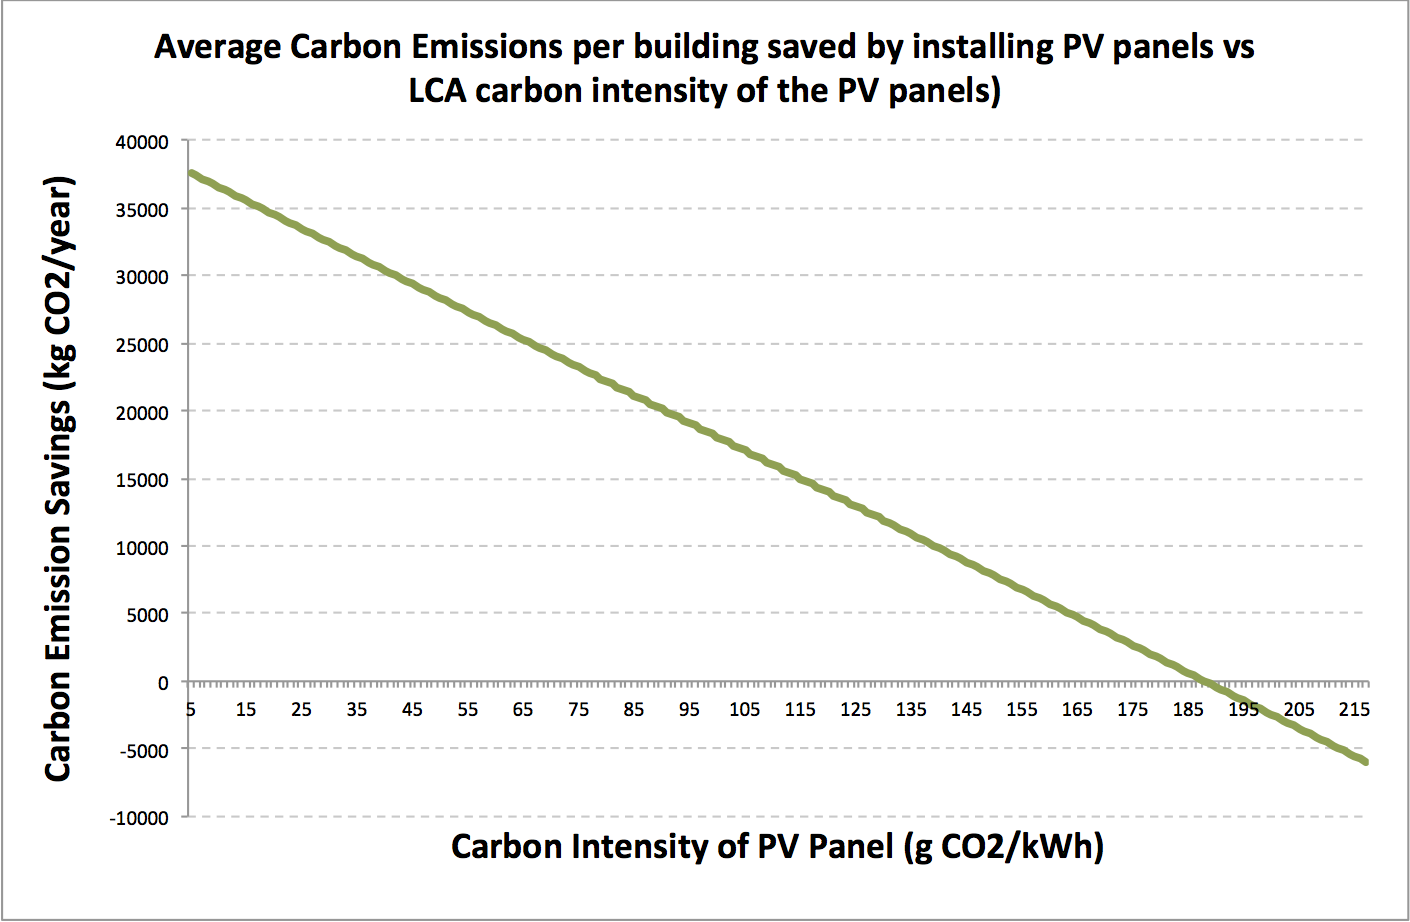
\includegraphics[scale=0.5]{pics/d6.png}
\caption{Average amount of carbon emissions saved vs. carbon intensity of PVCs, assuming a PVC efficiency of 16\% and 100\% of rooftop area utilization.}
\label{d6}
\end{center}
\end{figure}


\begin{figure}
\begin{center}
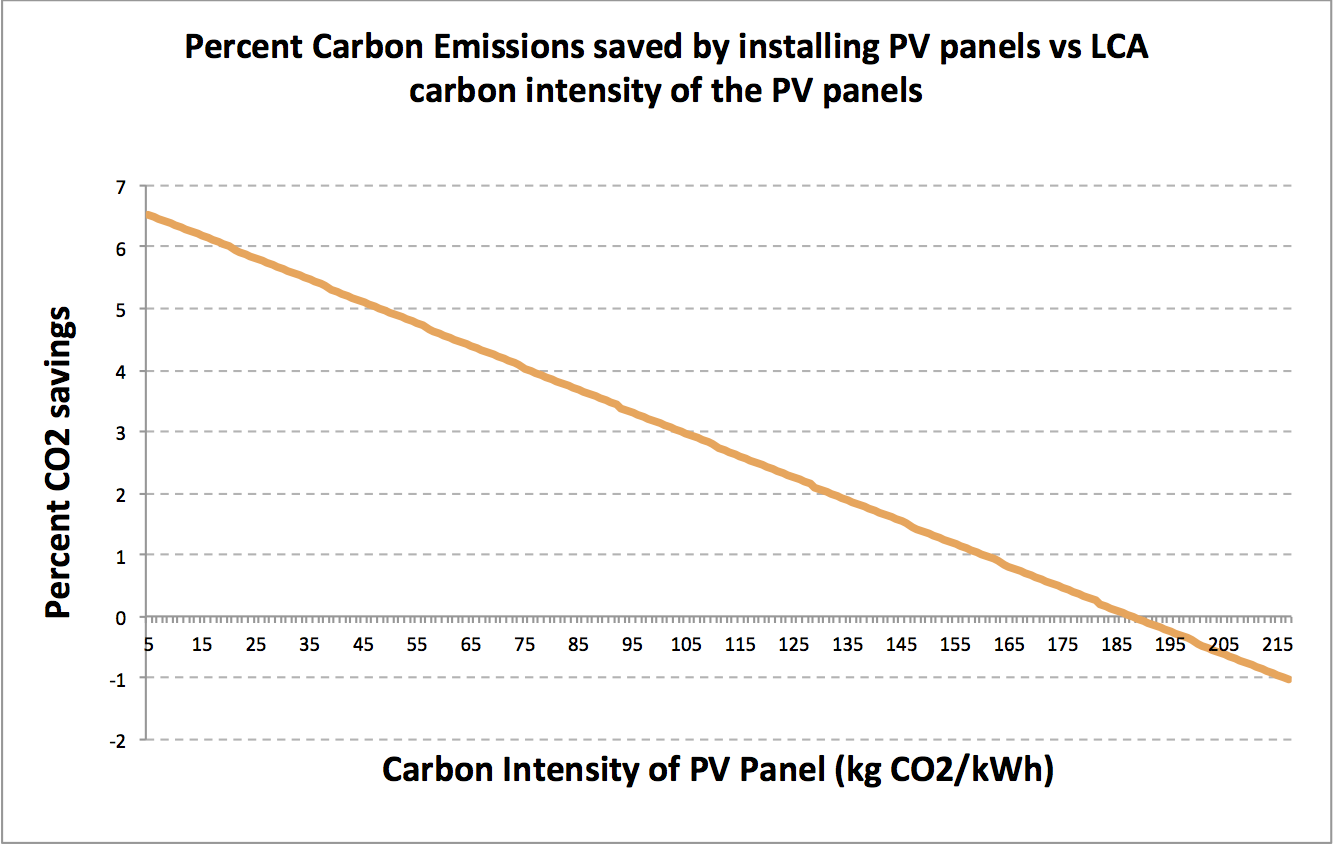
\includegraphics[scale=0.5]{pics/d7.png}
\caption{Percent of carbon emissions saved vs. carbon intensity of PVCs, assuming a PVC efficiency of 16\% and 100\% of rooftop area utilization.}
\label{d7}
\end{center}
\end{figure}


\begin{figure}
\begin{center}
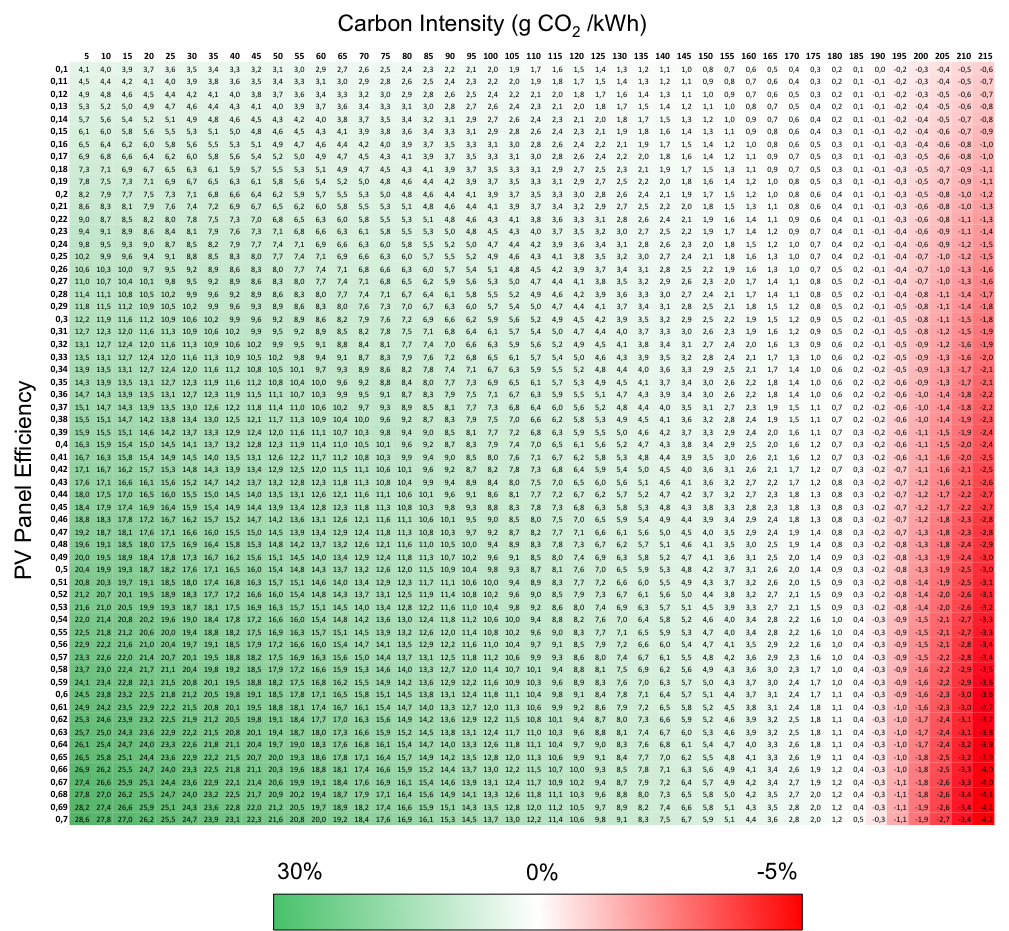
\includegraphics[scale=0.8]{pics/d8.png}
\caption{Heatmap of percent savings while varying carbon intensity (x-axis) and PVC efficiency (y-axis). Green represents positive savings and red represents negative savings.}
\label{d8}
\end{center}
\end{figure}


\subsection{Concluding Remarks}
The implementation of our policy could help address many of the Federal Government’s current goals of lowering its carbon emissions and increasing the fraction of renewable energy consumed by Federal buildings. This will, however, depend on the specifications of the solar panels being produced, in particular, the solar panel efficiency and the carbon intensity. Solar panels will have to be chosen carefully such that they improve carbon emissions and energy efficiency. This, in addition to helping the government meet its energy and emission goals (outlined above) will drive improvement of solar panel efficiency and carbon intensity, and thus drive the market forward.

